\documentclass{beamer}
\usepackage{graphicx}
\usepackage{braket}

\title{Quantum Support Vector Machine para Clasificación de Imágenes}
\author{Erick Jesús Ríos González}
\institute{Seminario de Redes Neuronales, UNAM}
\date{\today}

\begin{document}

% Slide 1: Título
\begin{frame}
    \titlepage
\end{frame}

% Slide 2: Introducción
\begin{frame}{Introducción}
    \begin{itemize}
        \item Las Support Vector Machines (SVM) son modelos de clasificación popular en aprendizaje automático.
        \item La Quantum Support Vector Machine (QSVM) introduce principios de computación cuántica para optimizar la clasificación en problemas complejos.
    \end{itemize}
\end{frame}

% Slide 3: Presentación de los Datos
\begin{frame}{Datos: Imágenes de Perros y Gatos}
    \begin{itemize}
        \item El conjunto de datos contiene imágenes etiquetadas de perros y gatos.
        \item Preprocesamiento: redimensionado, escalado y conversión a vectores de características.
        \item Los datos están divididos en conjuntos de entrenamiento y prueba.
    \end{itemize}
    \begin{figure}
        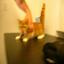
\includegraphics[scale=1]{../src/data/resized_images/cats/cat.0.jpg}
        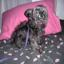
\includegraphics[scale=1]{../src/data/resized_images/dogs/dog.0.jpg}
        \caption{Ejemplos de imágenes de perros y gatos}
    \end{figure}
\end{frame}

% Slide 4: ¿Qué es una Support Vector Machine?
\begin{frame}{¿Qué es una Support Vector Machine?}
    \begin{itemize}
        \item Una SVM es un modelo supervisado que encuentra un hiperplano óptimo para clasificar datos en distintas clases.
        \item Se usa para problemas de clasificación y regresión.
        \item Ventaja: eficaz en conjuntos de datos de alta dimensión.
    \end{itemize}
    \begin{figure}
        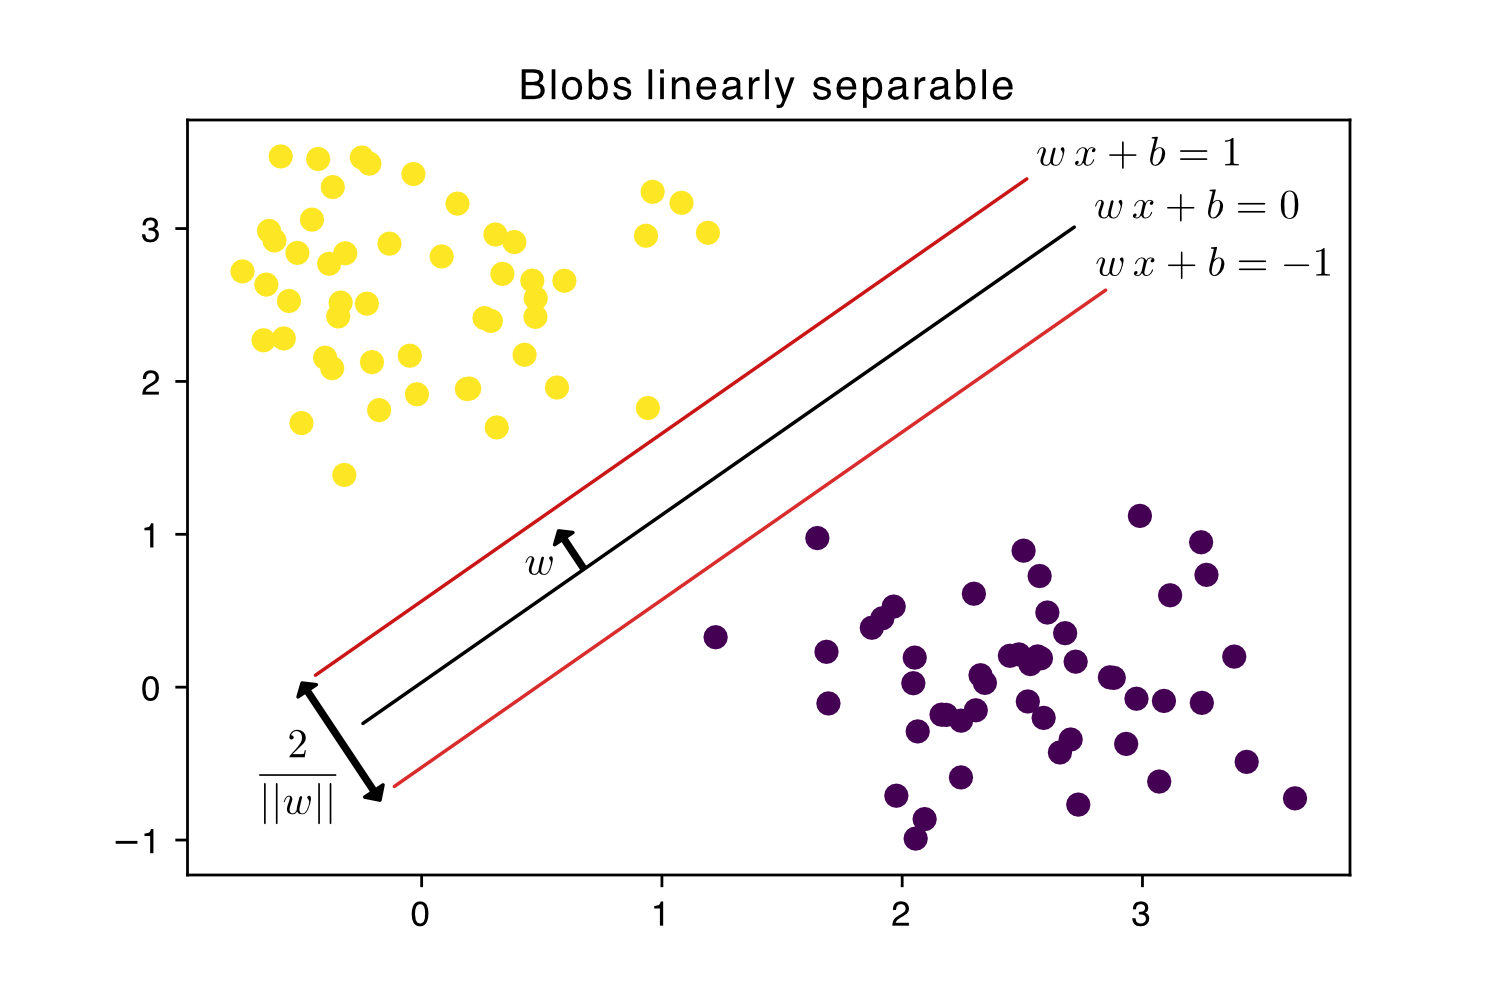
\includegraphics[width=0.6\textwidth]{../images/presentation/linear_svm_hardcore.png}
        \caption{Ilustración de una SVM}
    \end{figure}
\end{frame}

% Slide 5: ¿Qué es una Quantum Support Vector Machine?
\begin{frame}{¿Qué es una Quantum Support Vector Machine?}
    \begin{itemize}
        \item La QSVM es una versión cuántica de la SVM que utiliza principios de mecánica cuántica.
        \item Se implementa en circuitos cuánticos, aprovechando superposición y entrelazamiento para representar datos.
        \item Objetivo: mejorar la precisión en la clasificación de datos complejos y de alta dimensión.
    \end{itemize}
\end{frame}

% Slide 6: Funcionamiento de una QSVM
\begin{frame}{Funcionamiento de una QSVM}
    \begin{itemize}
        \item Recordemos que la idea de una SVM clasica es encontrar un hiperplano óptimo que separe un conjunto de puntos
        de otros. Puede ser lineal, pero tamibén puede ser más complejo.
        \item ¿Qué se necesita en el caso de una computadora cuántica?
        
    \end{itemize}
\end{frame}

\begin{frame}{¿Qué se necesita en el caso de una computadora cuántica?}
    \begin{itemize}
        \item Primero necesitamos calcular el vector de datos clasicos $\vec{x}$ en un vector cuántico $\ket{\Phi(\vec{x})}$.Esto lo conseguimos
        haciendo un circuito \(U_{\Phi(\vec{x})}\ket{0}\). Donde \(Phi()\) puede ser cualquier función clasica applicada en los datos clásicos $\vec{x}$.
        \item Luego necesitamos un circuito cuántica parametrizado \(W(\theta)\) que procese la informaciónde una forma en la que al final podamos aplicar medidas que regresen 
        \item 1 o -1 para cada entrada clásica de datos, lo cual va a identificar la etiqueta de la clase a la que pertenece.
    
    \end{itemize}
\end{frame}
\begin{frame}
    \begin{itemize}
        \item En el caso de una QSVM, el circuito cuántico solo usaremos mapas de características cuánticas \(U_{\Phi(\vec{x})}\) para mapear los datos clásicos a un espacio cuántico. Después
        construiremos el Kernel de la SVM con estos datos. Finalmnete calculando la matriz del kernel en una computadora cuántica podemos entrenar la QSVM de la misma forma que una clásica
        SVM.

    \end{itemize}
\end{frame}


\begin{frame}{Definición del Núcleo Cuántico}

    La idea del núcleo cuántico es la misma que en el caso clásico. Tomamos el producto interno, pero ahora con los mapas de características cuánticas.

    \textit{Nota:} No hay una prueba de que el QSVM ofrezca una ventaja cuántica, pero los autores de [1] argumentan que no habría ventaja si usamos mapas de características fáciles de simular clásicamente, ya que no necesitaríamos una computadora cuántica.

\end{frame}

% Slide 7: Resultados y Conclusiones
\begin{frame}{Resultados y Conclusiones}
    \begin{itemize}
        \item Precisión obtenida: 49.20\%. En análisis para mejorar con otros optimizadores.
        \item Conclusión: La QSVM muestra potencial, pero requiere ajustes adicionales para aplicaciones en imágenes.
        \item Futuro: Explorar optimizadores avanzados y configuraciones de circuitos cuánticos.
        \begin{figure}
            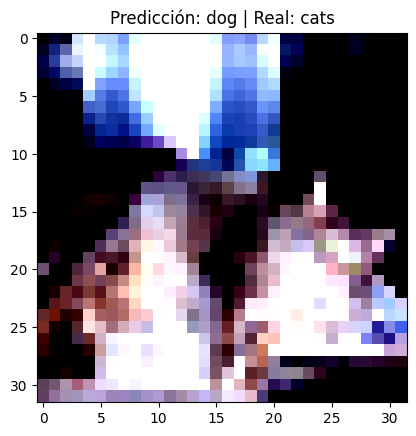
\includegraphics[width=0.2\textwidth]{../images/presentation/output.png}
            \caption{Predicción realizada por el primer modelo QSVM}
        \end{figure}
        \begin{figure}
            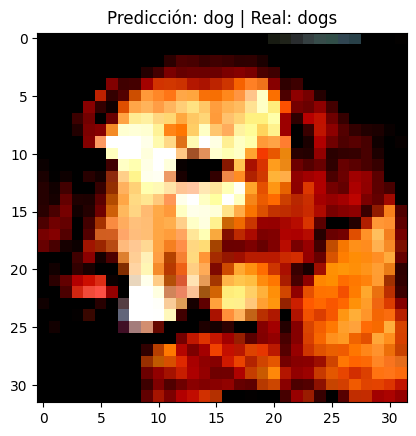
\includegraphics[width=0.2\textwidth]{../images/presentation/output2.png}
            \caption{Predicción realizada por el primer modelo QSVM}
        \end{figure}
    \end{itemize}
\end{frame}

\begin{frame}{Referencias}
    \begin{itemize}
        \item [1] Vojtech Havlicek, Antonio D. C'orcoles, Kristan Temme, Aram W. Harrow, Abhinav Kandala, Jerry M. Chow, and Jay M. Gambetta1, Supervised learning with quantum enhanced feature spaces, Nature 567, 209–212 (2019).

        \item [2] Rebentrost, P., Mohseni, M. \& Lloyd, S. Quantum support vector machine for big data classification, Physical review letters 113, 130503 (2014).
    \end{itemize}
\end{frame}
\end{document}
